\usepackage{graphicx}
%! Author = Philipp Emmenegger
%! Date = 08/06/2021

\section{Processes}
\subsection{1st Generation - Waterfall}
\begin{itemize}
    \item Split up development in independent steps
    \item Use specialized teams for every step
    \item Noticeable success rate for simple problems
\end{itemize}
\subsection{Problems}
\subsubsection{Software is rarely simple}
\begin{itemize}
    \item Simple problems are candidates for waterfall
    \item Chaotic problems are best avoided
    \item Complicated or Complex problems ask for more appropriate processes
\end{itemize}
\subsubsection{Too much uncertainty}
\begin{itemize}
    \item Giving reliable estimates at the beginning of a project is near impossible
    \item Uncertainty decreases over time
    \item Waterfall does not incorporate learning
\end{itemize}
\subsubsection{Lack of feedback}
\begin{itemize}
    \item Early changes are inexpensive
    \item Fast feedback is favorable
    \item Waterfall has no feedback cycles
    \item Problems might be detected very late
\end{itemize}
\subsubsection{No parallelization}
\begin{itemize}
    \item Sequential work is slow
    \item Parallelization should be strived
\end{itemize}
\subsubsection{Unused features}
\begin{itemize}
    \item Customers want features they rarely or never use
    \item Reasons: missing feedback cycles and lack of prioritization
\end{itemize}
\subsubsection{Knowledge loss on handovers}
\subsubsection{Missing autonomy}
\begin{itemize}
    \item Specialists get bored
    \item They rarely feel attached to the product
    \item Negative impact on the quality
\end{itemize}
\subsubsection{Sacrificing Quality}
\begin{itemize}
    \item Reducing efforts in implementation / testing to save time
    \item other phases already completed
\end{itemize}

\subsection{2nd Generation - Iterative and incremental}
\begin{itemize}
    \item Plan on different levels
    \item Do a little of everything at all time
    \item Incororate fast feedback
    \item Deliver working software after every iteration
    \item Enable cross-functional teams
\end{itemize}
\subsubsection{Main Criticism}
\begin{itemize}
    \item Too many documents
    \item Too complex process model
    \item missing tailoring
\end{itemize}

\subsection{3rd Generation - Agile Development}
\begin{itemize}
    \item Keep the benefits from 2nd generation
    \item Make processes slim and flexible
    \item Focus on delivering working software
\end{itemize}

\subsubsection{Agile Manifesto}
\begin{itemize}
    \item Individuals and interactions over processes and tools
    \item Working software over comprehensive documentation
    \item Customer collaboration over contract negotiation
    \item Responding to change over following a plan
\end{itemize}

\subsubsection{Core Principles}
\begin{itemize}
    \item Development is incremental
    \item Development is iterative
    \item Perform activities parallel
    \item Roles blur
    \item Planning is adaptive
    \item Scope can vary
    \item Requirements can change
    \item Working software as primary measure
    \item Document as you go
\end{itemize}

\subsubsection{Delivering working software}
\begin{itemize}
    \item An MVP has enough value that people are willing to use / buy it
    \item Demonstrates enough future benefit
    \item Provides feedback loop
    \item Prioritizing the backlog accordingly
    \item Creating MVP = creating vertical slices
    \item Every iteration, extend the previous slice further
    \item Cross-functional teams are best suited
    \item Reduces technical risks
\end{itemize}

\subsection{Scrum}
\textbf{Scrum Team}
\begin{itemize}
    \item Developers
    \item Product Owner
    \begin{itemize}
        \item Accountable for maximizing the value from the work of the team
        \item Accountable for effective Product Backlog management / prioritization
    \end{itemize}
    \item Scrum Master
    \begin{itemize}
        \item Accountable for establishing Scrum
        \item Accountable for the teams effectiveness
    \end{itemize}
\end{itemize}
\textbf{Scrum Events}
\begin{itemize}
    \item The Sprint (fixed length - one month or less)
    \item Sprint Planning
    \begin{itemize}
        \item Define a sprint goal
        \item Select items from the product backlog
        \item Decompose selected items into smaller work items
    \end{itemize}
    \item Daily Scrum
    \item Sprint Review
    \item Sprint Retrospective
\end{itemize}
\textbf{Scrum Artifacts}
\begin{itemize}
    \item Product Backlog
    \item Sprint Backlog
    \item Increment
\end{itemize}
\textbf{Scrum Values}
\begin{itemize}
    \item Commitment
    \item Focus
    \item Openness
    \item Respect Courage
\end{itemize}

\subsubsection{Measure Progress}
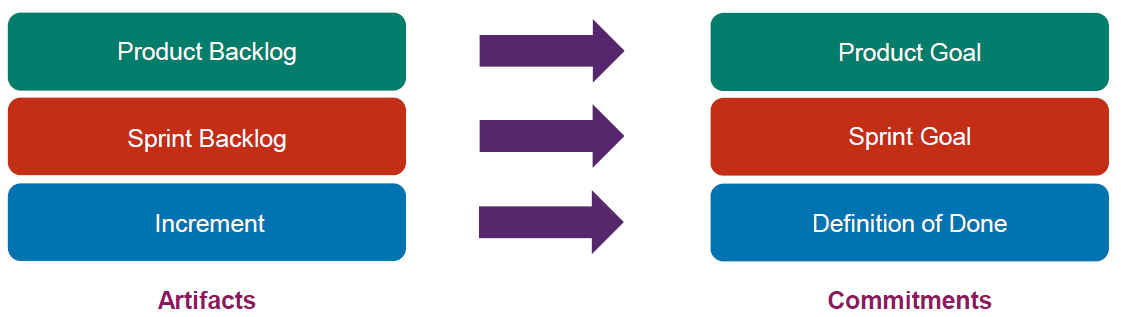
\includegraphics[width=\linewidth]{../img/scrum_progress.png}